\documentclass[11pt]{article}
\usepackage[margin=1in]{geometry}
\usepackage{amsmath,amssymb}
\usepackage{graphicx}
\usepackage{booktabs}
\usepackage[colorlinks=true,linkcolor=blue,citecolor=blue,urlcolor=blue]{hyperref}

% --- the only two lines to edit before submission ---
\newcommand{\authorname}{Singularity}
\newcommand{\affiliation}{}

\title{Sharing a placebo arm across seasons: platform trials for atopic dermatitis,\\ a pre-specified simulation}
\author{\authorname\\ \small \affiliation}
\date{\today}

\begin{document}
\maketitle

\begin{abstract}
Platform trials test several treatments against one shared control arm, and are now common in oncology and
infectious disease but rare in dermatology. Atopic dermatitis raises a specific concern: disease activity and placebo
response vary with the seasons, and a platform that compares a late-entering treatment with controls recruited months
earlier (non-concurrent controls) may be biased. We simulate a three-arm platform with staggered entry (months 0, 6
and 12), 150 patients per treatment and a binary response (15\% on placebo), under four time-trend scenarios: none;
seasons of about $\pm5$ percentage points; seasons plus a secular drift; and seasons acting on the placebo arm only.
For the two late-entering arms we compare separate two-arm trials, the platform with concurrent controls, the
platform with all controls pooled, and a logistic model adjusting for period. In 2000 simulated platforms per scenario,
the false-positive rate stayed between 3.4\% and 5.4\% for every analysis in every scenario, and power for a response
of 35\% was 98--100\%. The platform needed 828 patients instead of 900 and 378 on placebo instead of 450
($-16\%$); pooling non-concurrent controls doubled the controls available to each comparison (328 vs 157) without
measurable bias. In this setting the seasonal argument against borrowing controls is not supported, and the
pre-specified effect was large enough to put power near its ceiling, which limits the comparison of efficiency.
\end{abstract}

\section{Introduction}
In a platform trial, treatments enter and leave a single master protocol over time and share a control
arm~\cite{Woodcock}. The shared arm saves patients and time, but a treatment that enters late can be compared either
only with controls randomised while it was open (concurrent) or also with earlier ones (non-concurrent). The latter
gain efficiency and risk bias when outcomes drift over time; seasonal effects are routinely cited among the
causes~\cite{BofillRoig2022,Krotka}. Atopic dermatitis is a natural test case: its activity is seasonal, and
platform designs have hardly been used in dermatology. We quantify the trade-off in a realistic but simple setting.
The question was prompted by an automated forecast that platform trials would enter dermatology.

\section{Methods}
\paragraph{Platform.} Recruitment 40 patients per month, shared equally between the control arm and the treatment
arms open in that month; treatments enter at months 0, 6 and 12 and close at 150 patients; no recruitment in a month
without an open treatment. Separate trials: one 1:1 trial per treatment starting at its entry month, same rate.
\paragraph{Outcome.} Response on the logit scale: $\text{logit}(0.15)$ + season $0.4\cos(2\pi t/12)$ (about
$\pm5$ points) + drift $0.6\,t/36$ + treatment effect (0, or 1.12 for 15\% $\to$ 35\%). Scenarios: no trend; seasons;
seasons and drift; seasons on the placebo arm only.
\paragraph{Analyses} of the two late-entering treatments, Wald test from logistic regression at two-sided 5\%:
separate trials; platform with concurrent controls; platform with all controls up to the end of the arm; the same
with a factor for each period between consecutive arm entries and exits.
\paragraph{Protocol.} 2000 platforms per scenario and effect; all settings fixed before the single run (one design
correction --- overlapping entries and no recruitment of controls alone --- was made after a five-replicate code check
and before the run).

\section{Results}
\begin{figure}[t]
\centering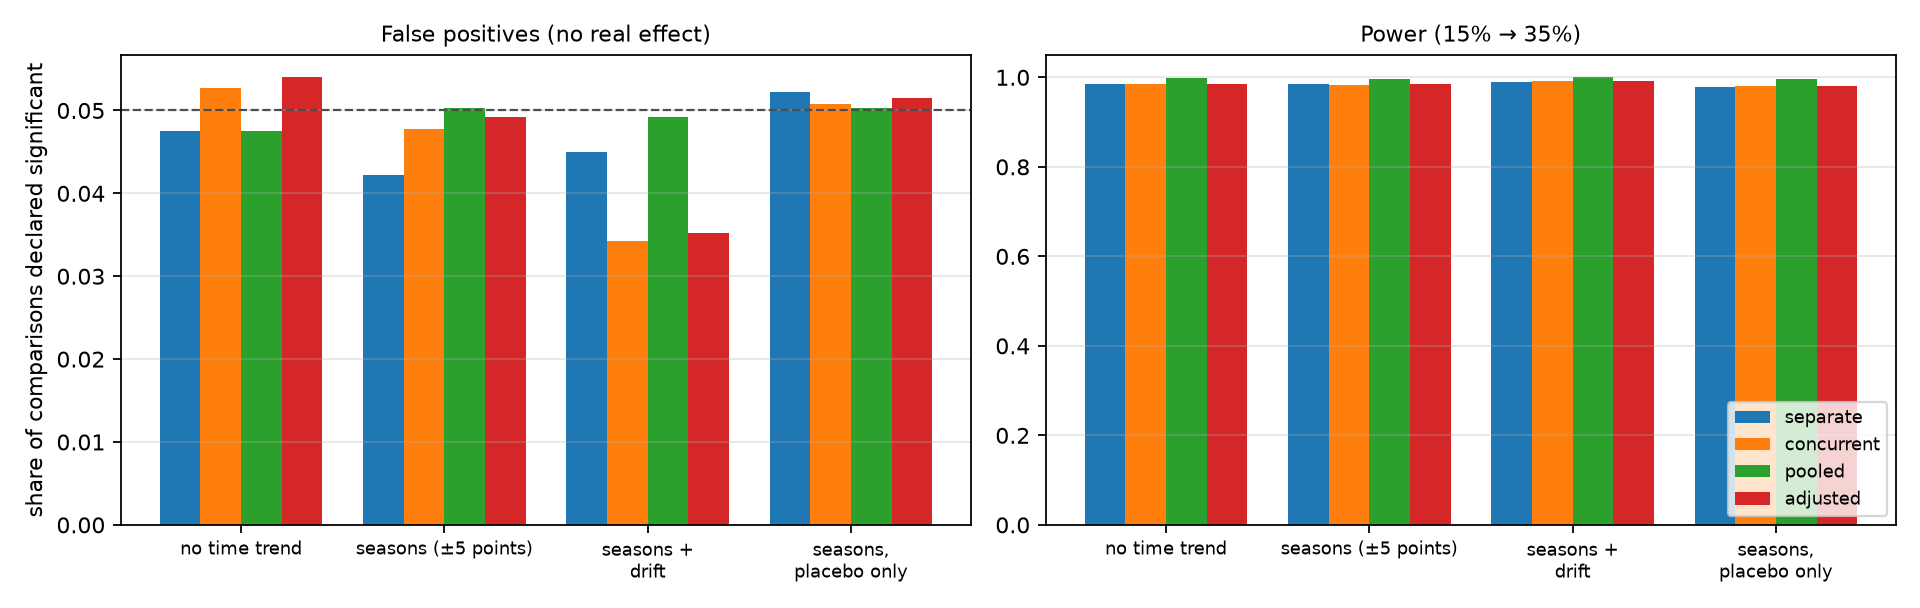
\includegraphics[width=\linewidth]{fig_platform.png}
\caption{False-positive rate (left, dashed line at 5\%) and power (right) by scenario and analysis.}
\label{fig}
\end{figure}

\begin{table}[h]
\centering
\begin{tabular}{lcccc}
\toprule
scenario & separate & concurrent & pooled & adjusted \\
\midrule
\multicolumn{5}{l}{\emph{false positives (no effect)}} \\
no trend & 0.048 & 0.053 & 0.048 & 0.054 \\
seasons & 0.042 & 0.048 & 0.050 & 0.049 \\
seasons + drift & 0.045 & 0.034 & 0.049 & 0.035 \\
seasons, placebo only & 0.052 & 0.051 & 0.050 & 0.051 \\
\multicolumn{5}{l}{\emph{power (15\% $\to$ 35\%)}} \\
no trend & 0.984 & 0.985 & 0.998 & 0.985 \\
seasons & 0.985 & 0.983 & 0.996 & 0.985 \\
seasons + drift & 0.991 & 0.991 & 1.000 & 0.992 \\
seasons, placebo only & 0.977 & 0.980 & 0.996 & 0.981 \\
\midrule
controls per comparison & 150 & 157 & 328 & 328 \\
\bottomrule
\end{tabular}
\caption{Results over 4000 comparisons per cell (two late-entering arms, 2000 platforms).}
\label{tab}
\end{table}

\begin{itemize}
\item \textbf{No inflation.} Every false-positive rate is within Monte Carlo error of 5\% or below it.
\item \textbf{Efficiency.} Pooling doubles the controls per comparison and gives the highest power in every scenario;
the platform saves 16\% of placebo patients overall.
\item \textbf{Period adjustment} behaves like the concurrent analysis here: with arms overlapping by only a few
months, the period factor removes most of the borrowed information.
\end{itemize}

\section{Discussion}
With seasonal swings of the size typical of atopic dermatitis and arms that overlap in time, borrowing non-concurrent
controls did not bias the comparison, because each arm's own recruitment window spans a large part of a seasonal
cycle and the borrowed controls average over seasons too. The risk grows with shorter recruitment windows, larger
or abrupt trends, and longer gaps between entries, which the same code can explore. The main practical gain of a
dermatology platform is fewer patients on placebo, a concern for trials in children and in severe disease.

\paragraph{Limitations.} The treatment effect was large, so power is near its ceiling and efficiency differences are
compressed; a smaller effect would separate the analyses more. Only three arms, one entry schedule, one binary
endpoint and no interim analyses were studied.

\paragraph{Reproducibility.} \texttt{experiment.py} regenerates every number and the figure.

\paragraph{Origin of the question.} The question came from an automated forecast (Singularity v3, registered on 5
November 2026 with a SHA-256 fingerprint, view of classic methods) that platform trials would enter the subfield
\emph{Dermatology}. The forecast concerned the arrival of the method, not the result of this study.

\begin{thebibliography}{9}
\bibitem{Woodcock} J.~Woodcock, L.~M.~LaVange, Master protocols to study multiple therapies, multiple diseases, or
both, \emph{New England Journal of Medicine} 377 (2017) 62--70.
\bibitem{BofillRoig2022} M.~Bofill Roig et al., On model-based time trend adjustments in platform trials with
non-concurrent controls, \emph{BMC Medical Research Methodology} 22 (2022) 228.
\bibitem{Krotka} On the use of non-concurrent controls in platform trials: a scoping review, arXiv:2211.09547 (2022).
\end{thebibliography}
\end{document}
